\chapter{Desarrollo de la Solución}
Dentro de esta sección se expone con precisión el procedimiento descrito previamente en la sección anterior, correspondiente a cada acción incluida en la metodología implementada, junto con los entregables previstos.

\section{Adquisición de los Datos}

\textbf{Actividad 1: Identificación de la data que contengan imágenes de rostros con características morfológicas faciales de proporciones similares}
 
Con el objetivo de entrenar un modelo de segmentación enfocado en características morfológicas faciales como arrugas y manchas, se llevó a cabo una exhaustiva búsqueda de bases de datos públicas en repositorios especializados. Se priorizó la recolección de conjuntos de datos que incluyeran imágenes faciales en alta resolución, variedad de edades, géneros y tonos de piel, así como condiciones de iluminación lo suficientemente controladas como para facilitar la segmentación de detalles faciales sutiles.

Durante este proceso, se identificaron diversos repositorios en plataformas como GitHub que ofrecían acceso a bases de datos con más de 200,000 imágenes faciales. Entre los conjuntos más destacados se encuentran versiones extendidas de datasets como CelebA, FFHQ (Flickr-Faces-HQ), y otros compendios curados por la comunidad investigadora, que contienen imágenes faciales etiquetadas o anotadas para tareas de reconocimiento y análisis facial.

Sin embargo, debido al enfoque específico de esta investigación la segmentación de características morfológicas finas como arrugas y manchas fue necesario realizar una selección cuidadosa de las imágenes más adecuadas. Para ello, se aplicaron criterios de claridad visual, resolución suficiente y visibilidad explícita de las deformaciones morfológicas faciales. Como resultado de este filtrado, se seleccionó un subconjunto compuesto por 5,000 imágenes faciales que cumplían con los siguientes criterios:

\begin{itemize}
    \item Alta calidad visual.   
    \item Visibilidad clara de texturas de la piel.
    \item Presencia evidente de arrugas y manchas.
    \item Proporciones faciales dentro de un rango estándar para facilitar el modelado.
\end{itemize} 

Este conjunto reducido pero representativo,lo podemos ver en la Figura \ref{4:fig1}, constituye la base de entrenamiento y validación del modelo propuesto. La selección manual de estos datos buscó optimizar el desempeño del modelo, al exponerlo exclusivamente a ejemplos que contienen información útil para aprender patrones asociados a las características morfológicas de interés.

\begin{figure}[h]
	\begin{center}
		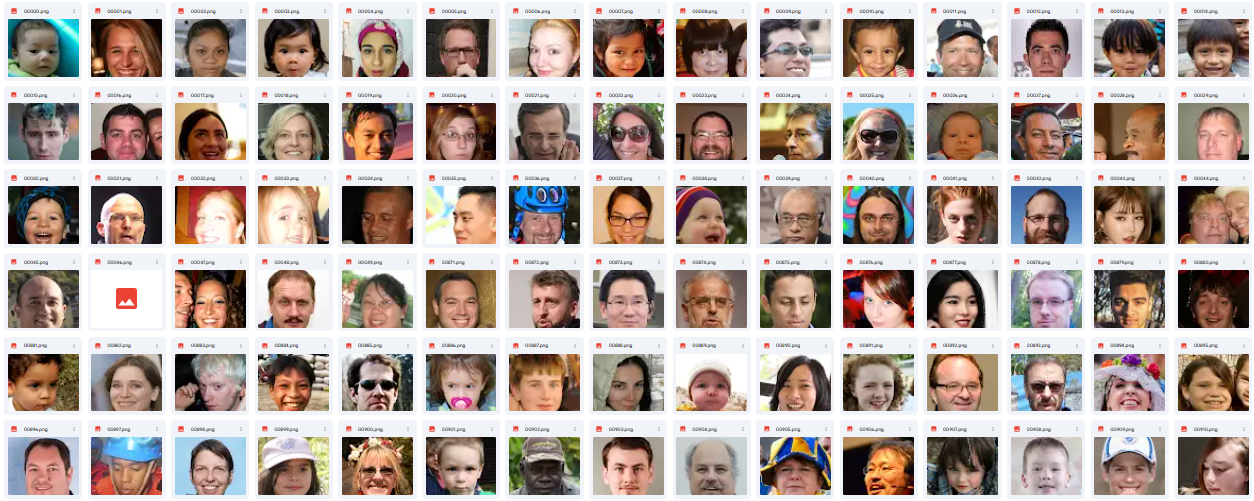
\includegraphics[width=0.75\textwidth]{4/figures/data.png}
		\caption[Dataset recolectado de repositorios]{Dataset recolectado de repositorios.\\
		Fuente: Elaboración propia}
		\label{4:fig1}
	\end{center}
\end{figure}

\section{Preprocesamiento de los Datos}

\textbf{Actividad 1: Filtración de imágenes faciales con características morfológicas}

Una vez recopilado el subconjunto de 5,000 imágenes faciales con características morfológicas visibles, se procedió a una etapa de filtración adicional orientada a reforzar la consistencia y la relevancia de los datos para la tarea de segmentación. Esta filtración se enfocó en garantizar que todas las imágenes seleccionadas contuvieran arrugas y manchas claramente identificables, descartando aquellas que, pese a su calidad visual, no presentaban estas características de manera explícita.

El proceso se realizó mediante una inspección semiautomática, apoyada en técnicas básicas de detección de texturas y realce de bordes para facilitar la identificación visual de las zonas con deformaciones. Como resultado, se aseguraron condiciones homogéneas entre las imágenes del dataset final, lo que permitió una base sólida para la generación de máscaras de segmentación precisas.

\textbf{Actividad 2: Representación y normalización de las imágenes faciales}

Con el conjunto de imágenes definitivo, se ejecutó un proceso de preprocesamiento estandarizado con dos objetivos principales: uniformar las dimensiones espaciales de las imágenes y generar las máscaras binarias asociadas a las regiones con deformaciones morfológicas.

En primer lugar, todas las imágenes fueron redimensionadas a una resolución uniforme de 1024x1024 píxeles, preservando la relación de aspecto y aplicando interpolación bilineal para mantener la calidad visual. Esta estandarización es fundamental para asegurar la compatibilidad estructural con las redes neuronales convolucionales utilizadas en etapas posteriores, y facilita la aplicación de operaciones convolucionales sobre áreas homogéneas.

En segundo lugar, se generaron máscaras binarias (en blanco y negro) correspondientes a cada imagen. Estas máscaras representan las regiones específicas del rostro que contienen arrugas, manchas u otras alteraciones morfológicas, codificadas de la siguiente manera:

\begin{itemize}
    \item Blanco (valor 1): Regiones con características morfológicas relevantes (objetivo de segmentación).   
    \item Negro (valor 0): Regiones sin interés morfológico.
\end{itemize} 

Las máscaras, como se ve en la Figura \ref{4:fig2}, fueron elaboradas a partir de una combinación de anotación semiautomática y herramientas de realce de texturas, contrastes y gradientes, con verificación manual en una muestra aleatoria para asegurar su validez.

\begin{figure}[h]
	\begin{center}
		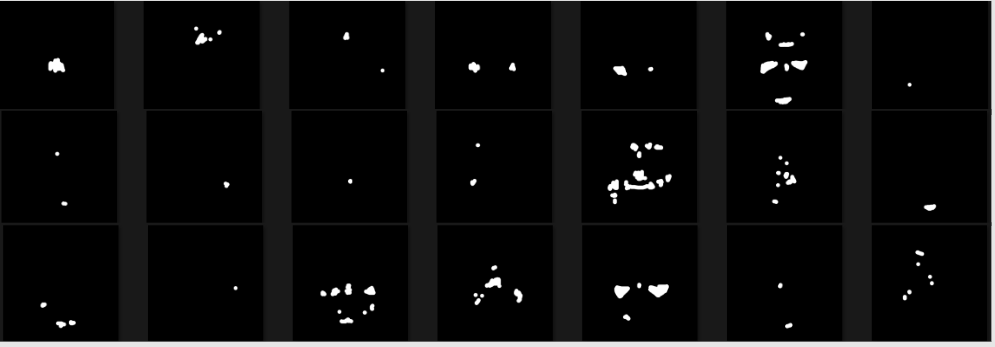
\includegraphics[width=0.75\textwidth]{4/figures/mascaras.png}
		\caption[Máscaras binarias generadas]{Máscaras binarias generadas.\\
		Fuente: Elaboración propia}
		\label{4:fig2}
	\end{center}
\end{figure}

Este proceso de representación y normalización, como se ve en el diagrama final de Preprocesamiento en la Figura \ref{4:fig3}, permitió convertir los datos originales en pares de entrada (imagen facial) y salida (máscara de segmentación), aptos para el entrenamiento supervisado del modelo de segmentación basado en redes neuronales convolucionales.

\begin{figure}[h]
	\begin{center}
		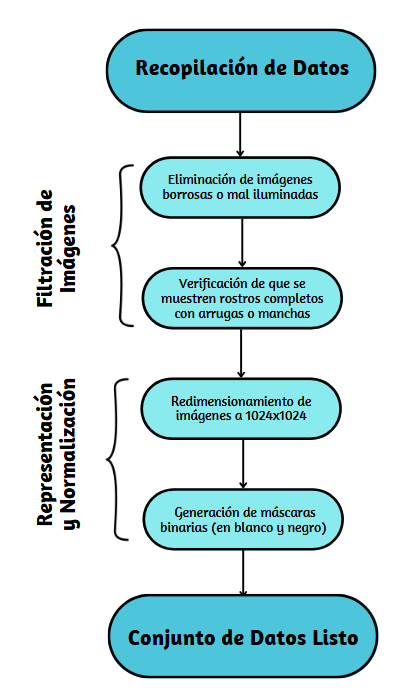
\includegraphics[width=0.45\textwidth]{4/figures/diagrama final prepo.png}
		\caption[Diagrama de Preprocesamiento Utilizado]{Diagrama de Preprocesamiento Utilizado.\\
		Fuente: Elaboración propia}
		\label{4:fig3}
	\end{center}
\end{figure}
\newpage
\section{Desarrollo de los Modelos de Segmentación}

\begin{enumerate}
  \item \textbf{Modelo de Segmentación: U-Net}
  \begin{itemize}
  \item\textbf{Actividad 1: Diseño de la arquitectura del modelo}
  El modelo implementado es una arquitectura de red neuronal convolucional U-Net, que es comúnmente utilizada para tareas de segmentación de imágenes. Esta red se caracteriza por su estructura simétrica, compuesta por una parte de codificación (encoder) y decodificación (decoder), con conexiones de salto (skip connections) entre ellas. El objetivo principal de la U-Net es capturar características de bajo y alto nivel, y luego reconstruir la imagen segmentada a partir de esas características.

\textbf{Estructura del Modelo}

La arquitectura de la U-Net se puede dividir en dos fases principales: la fase de codificación (encoder) y la fase de decodificación (decoder).

\textbf{Bloques de Convolución}

Cada bloque de convolución en el encoder y el decoder sigue el mismo patrón. Un bloque está compuesto por:
\begin{itemize}
    \item Dos capas de convolución, cada una seguida por \texttt{BatchNorm2d} (normalización por lotes) y \texttt{ReLU} (función de activación).
    \item La normalización por lotes ayuda a estabilizar y acelerar el entrenamiento, mientras que la activación ReLU introduce no linealidad al modelo.
    \item Las capas de convolución utilizan un tamaño de filtro de $3 \times 3$, lo que significa que cada capa de convolución opera sobre una vecindad local de 3 píxeles en la imagen de entrada.
\end{itemize}

\textbf{Encoder (Codificador)}

El encoder está diseñado para extraer características de la imagen a través de una serie de capas convolucionales. En cada paso, la imagen es reducida en resolución mediante el uso de max pooling, lo que permite que la red capture información contextual en escalas de mayor nivel.

\begin{itemize}
    \item \textbf{Encoder 1}: La imagen de entrada con 3 canales (RGB) pasa a través del primer bloque de convolución, produciendo 64 mapas de características. Luego, se aplica un max pooling para reducir la resolución de la imagen a la mitad.
    \item \textbf{Encoder 2}: Los 64 mapas de características se procesan en el segundo bloque de convolución, produciendo 128 mapas de características. También se aplica max pooling para reducir la resolución.
    \item \textbf{Encoder 3}: Los 128 mapas de características se procesan en el tercer bloque de convolución, produciendo 256 mapas de características, seguidos por max pooling.
    \item \textbf{Encoder 4}: Los 256 mapas de características se procesan en el cuarto bloque de convolución, produciendo 512 mapas de características, seguidos por max pooling.
\end{itemize}

\textbf{Bottleneck}

En esta etapa, la red alcanza su máxima abstracción. El bottleneck se compone de un bloque de convolución que aumenta la profundidad a 1024 mapas de características. A diferencia de los bloques anteriores, esta parte no aplica max pooling, pero se realiza una convolución estándar. Aquí, la resolución de la imagen se mantiene constante para preservar la información de alto nivel.

\textbf{Decoder (Decodificador)}

El decoder tiene como objetivo reconstruir la imagen segmentada a partir de la representación abstracta generada en el bottleneck. El proceso se realiza mediante convoluciones transpuestas (también conocidas como deconvoluciones), que aumentan la resolución de las características. Además, se utilizan conexiones de salto (skip connections) para combinar la información de alta resolución del encoder con la información generada en el decoder.

\begin{itemize}
    \item \textbf{Upconv4 y Decoder 4}: La salida del bottleneck (1024 mapas de características) se expande utilizando una convolución transpuesta (upconv4), lo que duplica la resolución de la imagen. Luego, esta salida se concatena con los 512 mapas de características de \texttt{enc4}. El resultado se pasa a través de un bloque convolucional (dec4), manteniendo la cantidad de mapas en 512.
    \item \textbf{Upconv3 y Decoder 3}: De manera similar, se aplica una convolución transpuesta (upconv3) que aumenta la resolución de la imagen a la mitad de su tamaño original. Se concatena con los 256 mapas de características de \texttt{enc3} y se pasa por un bloque convolucional (dec3).
    \item \textbf{Upconv2 y Decoder 2}: La resolución de la imagen se duplica nuevamente usando upconv2, y se concatena con los 128 mapas de características de \texttt{enc2}. El resultado se procesa en dec2.
    \item \textbf{Upconv1 y Decoder 1}: Finalmente, se utiliza upconv1 para duplicar la resolución a su tamaño original. Los 64 mapas de características generados en \texttt{enc1} se concatenan con la salida de upconv1 y se pasan a través de dec1.
\end{itemize}

\textbf{Capa Final}

La salida final de la red se genera aplicando una convolución $1 \times 1$. Esta capa reduce el número de canales de 64 a la cantidad deseada de canales en la salida (por ejemplo, 3 para una imagen RGB segmentada). La convolución de $1 \times 1$ permite realizar una clasificación de cada píxel de la imagen.

\textbf{Funcionamiento General}

\begin{itemize}
    \item La imagen de entrada pasa por el encoder, donde se extraen características a diferentes escalas. La resolución de la imagen se reduce en cada paso utilizando max pooling, y la profundidad de los mapas de características aumenta.
    \item En el bottleneck, se extrae la representación más abstracta de la imagen, utilizando un bloque convolucional sin max pooling.
    \item El decoder aumenta la resolución de la imagen utilizando convoluciones transpuestas, y las conexiones de salto (skip connections) se utilizan para combinar las características de bajo nivel del encoder con las características de alto nivel del decoder.
    \item Finalmente, una capa de convolución $1 \times 1$ genera la salida segmentada de la red.
\end{itemize}

\textbf{Pseudocódigo del Modelo}

\begin{verbatim}
Input: Imagen X (3 canales)

e1 = enc1(X)  # Primer bloque de convolución
e2 = enc2(pool1(e1))  # Segundo bloque de convolución
e3 = enc3(pool2(e2))  # Tercer bloque de convolución
e4 = enc4(pool3(e3))  # Cuarto bloque de convolución

b = bottleneck(pool4(e4))  # Bottleneck, no max pooling

d4 = upconv4(b)  # Expansión con convolución transpuesta
d4 = dec4(concat(d4, e4))  # Conexión de salto con e4
d3 = upconv3(d4)  # Expansión con convolución transpuesta
d3 = dec3(concat(d3, e3))  # Conexión de salto con e3
d2 = upconv2(d3)  # Expansión con convolución transpuesta
d2 = dec2(concat(d2, e2))  # Conexión de salto con e2
d1 = upconv1(d2)  # Expansión con convolución transpuesta
d1 = dec1(concat(d1, e1))  # Conexión de salto con e1

Output = final_conv(d1)  # Capa final de convolución
\end{verbatim}


  \item\textbf{Actividad 2: Definición de componentes del modelo}
  \begin{itemize}
    \item \textbf{Clase \texttt{SegmentacionMulticlaseDataset}}: Esta clase personalizada hereda de \texttt{torch.utils.data.Dataset} y se encarga de cargar imágenes de entrada (rostros) y sus correspondientes máscaras binarias (arrugas y manchas). Se generan máscaras multiclase fusionando las siguientes clases:
    \begin{itemize}
        \item Clase 0: Fondo (valor por defecto en la máscara).
        \item Clase 1: Arrugas (píxeles donde la imagen de arrugas tenga valores mayores a 50).
        \item Clase 2: Manchas (píxeles donde la imagen de manchas tenga valores mayores a 50).
    \end{itemize}
    Para el preprocesamiento se utiliza la librería Albumentations. Las transformaciones incluyen:
    \begin{itemize}
        \item \texttt{HorizontalFlip(p=0.5)}
        \item \texttt{Rotate(limit=10, p=0.3)}
        \item \texttt{RandomBrightnessContrast(p=0.3)}
        \item \texttt{Resize(256, 256)}
        \item \texttt{ToTensorV2()}
    \end{itemize}
    Esto permite robustecer el modelo contra pequeñas variaciones geométricas e iluminación.

    \item \textbf{Modelo \texttt{UNet}}: Arquitectura de segmentación semántica basada en una estructura en forma de U. Se compone de dos fases principales:
    \begin{itemize}
        \item \textbf{Codificador (Encoder):} Reduce progresivamente la dimensión espacial mientras aumenta la profundidad de características:
        \begin{itemize}
            \item \texttt{enc1}: \( \text{Conv2d}(3 \rightarrow 64) \rightarrow \text{BN} \rightarrow \text{ReLU} \rightarrow \text{Conv2d}(64 \rightarrow 64) \rightarrow \text{BN} \rightarrow \text{ReLU} \)
            \item \texttt{pool1}: MaxPool \(2 \times 2\)
            \item \texttt{enc2}: \(64 \rightarrow 128\), seguido de \texttt{pool2}, etc.
        \end{itemize}
        \item \textbf{Cuello de botella (Bottleneck):} Capa de mayor profundidad \(512 \rightarrow 1024\), sin reducción espacial.
        \item \textbf{Decodificador (Decoder):} Recupera resolución espacial mediante \texttt{ConvTranspose2d} (upsampling) y concatenación con las salidas del encoder (skip connections). Cada bloque incluye dos capas convolucionales como el encoder.
        \item \textbf{Capa final:} Una convolución \(1 \times 1\) que transforma el mapa de características final (con 64 canales) en un tensor con 3 canales de salida (uno por clase).
    \end{itemize}
\end{itemize}
\end{itemize}

\vspace{1em}
\textbf{Resumen de interacción entre componentes:}

\begin{itemize}
    \item El conjunto de datos genera muestras de entrenamiento y validación a partir de rutas de imágenes faciales y sus respectivas máscaras binarias.
    \item Las imágenes se transforman y normalizan en el rango \([0, 1]\) y se convierten en tensores \texttt{float}.
    \item La máscara multiclase (valores en \{0,1,2\}) es convertida en tipo \texttt{long} para ser compatible con \texttt{nn.CrossEntropyLoss}.
    \item El modelo UNet recibe un batch de imágenes y predice un tensor de salida con forma \((B, C, H, W)\), donde \(C = 3\).
    \item Se calcula la pérdida ponderada y se retropropaga para actualizar los pesos.
    \item En validación, se observa la capacidad del modelo para distinguir fondo, arrugas y manchas en imágenes no vistas.
\end{itemize}


  \item \textbf{Modelo de Segmentación: U-Net Attention}
  \begin{itemize}
  \item\textbf{Actividad 1: Diseño de la arquitectura del modelo}
  La arquitectura propuesta se basa en el modelo \textbf{U-Net con mecanismos de atención} (\texttt{UNetAttention}), que combina una red convolucional simétrica tipo encoder-decoder con puertas de atención (\texttt{AttentionGate}) para mejorar el enfoque en las regiones relevantes de la imagen.

\textbf{Encoder (Codificador)}
El encoder está diseñado para capturar características de bajo a alto nivel a partir de la imagen de entrada. Consiste en cuatro bloques llamados \texttt{DoubleConv}:
\begin{itemize}
    \item \textbf{Encoder 1}: Dos convoluciones $3\times3$ (con \texttt{padding}=1), normalización por lotes (BatchNorm) y activación ReLU. Extrae características básicas (bordes, texturas) de las entradas con 3 canales (RGB) y produce 64 mapas de características.
    \item \textbf{Encoder 2}: Similar al anterior, pero recibe 64 mapas y genera 128, aumentando la capacidad de representación.
    \item \textbf{Encoder 3}: Pasa de 128 a 256 mapas, detectando patrones más complejos.
    \item \textbf{Encoder 4}: Pasa de 256 a 512 mapas, capturando características globales.
\end{itemize}
Cada bloque está seguido de una capa \texttt{MaxPool2d(2)}, que reduce la resolución a la mitad e incrementa el campo receptivo, permitiendo captar relaciones espaciales más amplias.

\textbf{Puente (Bottleneck)}
Entre el encoder y el decoder se encuentra el \textbf{bottleneck}, otra capa \texttt{DoubleConv} que recibe 512 mapas y genera 1024. Esta parte actúa como un resumen altamente condensado de toda la información, crucial para sintetizar las representaciones aprendidas antes de reconstruirlas.

\textbf{Attention Gates (Puertas de Atención)}
En lugar de pasar directamente los mapas del encoder al decoder (skip connections), se introducen mecanismos de atención:
\begin{itemize}
    \item Cada \texttt{AttentionGate} recibe dos entradas: $g$ (señal del decoder) y $x$ (señal del encoder).
    \item Ambas se alinean en dimensiones espaciales y se transforman con convoluciones $1\times1$ para reducir canales.
    \item La suma de ambas se activa con ReLU, pasa por otra convolución $1\times1$, BatchNorm y una función sigmoide, generando un mapa de atención $\psi$ entre 0 y 1.
    \item Finalmente, $\psi$ se multiplica por la señal $x$ para filtrar solo las características relevantes.
\end{itemize}
Esto asegura que solo la información útil del encoder fluya al decoder, reduciendo el ruido y enfocándose en las regiones clave.

\textbf{Decoder (Decodificador)}
El decoder reconstruye la imagen segmentada paso a paso:
\begin{itemize}
    \item \textbf{Upconv4}: Upsampling (\texttt{ConvTranspose2d}) de 1024 a 512, concatenado con la salida del encoder4 filtrado por la atención (att3).
    \item \textbf{Decoder4}: \texttt{DoubleConv} que procesa los 1024 canales concatenados y produce 512.
    \item \textbf{Upconv3}, \textbf{Decoder3}: De 512 a 256, concatenado con att2, procesado a 256.
    \item \textbf{Upconv2}, \textbf{Decoder2}: De 256 a 128, concatenado con att1, procesado a 128.
    \item \textbf{Upconv1}, \textbf{Decoder1}: De 128 a 64, concatenado con enc1 (sin atención), procesado a 64.
\end{itemize}

\textbf{Capa Final}
La capa final es una convolución $1\times1$ que reduce los 64 mapas de características a un solo canal de salida (\texttt{out\_channels=1}), generando el mapa binario segmentado.

\textbf{Razones del Diseño}
\begin{itemize}
    \item \textbf{Convoluciones dobles}: Mejoran la capacidad de aprendizaje local sin aumentar demasiado la profundidad.
    \item \textbf{BatchNorm}: Acelera la convergencia y estabiliza el entrenamiento.
    \item \textbf{Atención}: Permite que el modelo se enfoque en las regiones importantes, evitando pasar ruido del encoder al decoder.
    \item \textbf{Skip connections}: Ayudan a recuperar detalles espaciales perdidos por el pooling.
    \item \textbf{Puertas de atención}: Añaden un mecanismo de filtrado adaptativo, crucial en tareas donde no toda la información del encoder es igualmente relevante.
    \item \textbf{Upsampling con transposed convolutions}: Permite recuperar resolución espacial de manera más precisa que el simple escalado.
\end{itemize}

\textbf{Detalle del Funcionamiento}
El proceso completo del modelo se detalla de la siguiente manera:
\begin{itemize}
\item La imagen de entrada se procesa a través del encoder, extrayendo características jerárquicas que van desde bordes simples hasta patrones complejos, reduciendo la resolución pero aumentando la abstracción.
\item El bottleneck actúa como un cuello de botella que condensa toda la información del encoder en una representación compacta y de alto nivel.
\item El decoder empieza a recuperar la resolución original usando operaciones de upsampling, reconstruyendo progresivamente el mapa segmentado.
\item En cada paso del decoder, las características recuperadas se enriquecen mediante la concatenación de información relevante proveniente del encoder, filtrada cuidadosamente por las puertas de atención.
\item Las puertas de atención permiten que el modelo ignore información irrelevante y se enfoque en regiones específicas de interés para la tarea de segmentación.
\item Finalmente, la capa de salida transforma las características finales en una máscara binaria que identifica las regiones segmentadas de interés en la imagen.
\end{itemize}

Este funcionamiento asegura que el modelo combine detalles locales finos con contexto global y mecanismos de relevancia, logrando una segmentación precisa y robusta.

\textbf{Pseudocódigo del Modelo}
\begin{verbatim}
Input: Imagen X

# Encoder
enc1 = DoubleConv(X)
enc2 = DoubleConv(MaxPool(enc1))
enc3 = DoubleConv(MaxPool(enc2))
enc4 = DoubleConv(MaxPool(enc3))

# Bottleneck
bottleneck = DoubleConv(MaxPool(enc4))

# Decoder con atención
up4 = UpConv(bottleneck)
att3 = AttentionGate(up4, enc4)
up4_cat = Concatenate(up4, att3)
dec4 = DoubleConv(up4_cat)

up3 = UpConv(dec4)
att2 = AttentionGate(up3, enc3)
up3_cat = Concatenate(up3, att2)
dec3 = DoubleConv(up3_cat)

up2 = UpConv(dec3)
att1 = AttentionGate(up2, enc2)
up2_cat = Concatenate(up2, att1)
dec2 = DoubleConv(up2_cat)

up1 = UpConv(dec2)
up1_cat = Concatenate(up1, enc1)
dec1 = DoubleConv(up1_cat)

# Salida final
Output = Conv1x1(dec1)
Return Output
\end{verbatim}

  \item\textbf{Actividad 2: Definición de componentes del modelo}

  En esta actividad se definen los módulos fundamentales y los elementos de entrenamiento que constituyen el modelo UNetAttention. A continuación se describe en detalle cada uno:

\textbf{Módulos arquitectónicos}

\begin{itemize}
\item \textbf{DoubleConv}:
Es un bloque formado por dos capas convolucionales secuenciales, cada una seguida de Batch Normalization y activación ReLU.
Este bloque permite:
\begin{itemize}
\item Extraer patrones locales en múltiples niveles.
\item Evitar problemas de saturación o desaparición de gradientes gracias a ReLU.
\item Estabilizar y acelerar el entrenamiento mediante BatchNorm, que normaliza las salidas y reduce la dependencia de la inicialización.
\end{itemize}

\item \textbf{AttentionGate}:
Es un módulo que implementa un mecanismo de atención espacial. Su estructura:
\begin{itemize}
\item Dos entradas: 
$\mathbf{x}$ (del encoder) y $\mathbf{g}$ (del decoder)

g (del decoder).
\item Aplicación de convoluciones 
1
×
1
1×1 para reducir dimensionalidad.
\item Suma de las dos señales transformadas y paso por activación ReLU.
\item Otra convolución 
1
×
1
1×1 seguida de BatchNorm y activación Sigmoid, que genera un mapa de atención 
\item Multiplicación punto a punto de $\psi$ con $\mathbf{x}$, filtrando las características relevantes.

x, filtrando las características relevantes.
\end{itemize}
El objetivo es permitir al modelo “enfocarse” solo en las regiones de interés para la tarea de segmentación, reduciendo ruido y mejorando la precisión espacial.

\item \textbf{UpConv (Transposed Convolution)}:
Operación que realiza upsampling aprendido, permitiendo reconstruir la resolución espacial en el decoder. Es superior al upsampling por interpolación porque también aprende qué características son importantes al expandir.

\item \textbf{Conv1x1 final}:
Capa de convolución 
1
×
1
1×1 que reduce los canales finales a uno solo (para segmentación binaria), generando la máscara final.
\end{itemize}



\textbf{Resumen de interacción entre componentes}
Durante el entrenamiento:
\begin{itemize}
\item El modelo recibe imágenes de entrada que son procesadas por los módulos convolucionales y de atención.
\item Las predicciones por píxel son comparadas contra las máscaras reales usando la función de pérdida ponderada.
\item El optimizador AdamW ajusta los pesos del modelo minimizando la pérdida.
\item El scheduler supervisa la evolución de la métrica de validación y adapta la tasa de aprendizaje si es necesario.
\end{itemize}

Este conjunto de componentes fue seleccionado cuidadosamente para equilibrar capacidad, estabilidad, precisión y generalización.

  \end{itemize}
  \item \textbf{Modelo de Segmentación: U-Net con codificador MiT-B0 (Mix Transformer)}
  \begin{itemize}
  \item\textbf{Actividad 1: Diseño de la arquitectura del modelo}
  El modelo \texttt{MiT-B0} (Mix Transformer) es una arquitectura de red neuronal que combina la estructura de U-Net con bloques de atención de tipo Transformer. Esta combinación permite al modelo capturar tanto características locales como globales en las imágenes, mejorando la segmentación en comparación con arquitecturas convencionales.
\textbf{Estructura del modelo}
\begin{itemize}
  \item \textbf{Encoder (Codificador)}:  
    Se utiliza un backbone \texttt{MiT-B0} preentrenado en ImageNet como codificador. Este encoder está compuesto por cuatro etapas jerárquicas de procesamiento:
    \begin{itemize}
      \item Etapa 1: recibe la imagen de entrada $X\in\mathbb{R}^{H\times W\times3}$ y produce un mapa de características de dimensión $\frac{H}{4}\times\frac{W}{4}\times C_1$.
      \item Etapa 2: reduce la resolución a $\frac{H}{8}\times\frac{W}{8}$ y aumenta la profundidad a $C_2$ canales.
      \item Etapa 3: genera un mapa de $\frac{H}{16}\times\frac{W}{16}\times C_3$.
      \item Etapa 4: produce la salida más profunda del encoder, de tamaño $\frac{H}{32}\times\frac{W}{32}\times C_4$.
    \end{itemize}
    Cada etapa combina proyecciones lineales y mecanismos de auto‑atención eficiente, capturando relaciones espaciales y contextuales tanto locales como globales. Las salidas intermedias de cada etapa se guardan para las conexiones de salto.

  \item \textbf{Bottleneck}:  
    Conceptualmente corresponde al punto más profundo de la U‑Net, situado justo después de la cuarta etapa del encoder. Aquí en la fórmula \ref{eq:bottleneck_mapa}, las características están más condensadas y contienen la máxima abstracción:
    \begin{equation}\label{eq:bottleneck_mapa}
      \text{Bottleneck} = \text{FeatureMap}_{4} \in \mathbb{R}^{\frac{H}{32}\times\frac{W}{32}\times C_4}.
  \end{equation}
  \myequations{Cuarto mapa de características (Bottleneck)}

    Aunque no se añade un bloque explícito adicional, esta representación se considera el “cuello de botella” antes de iniciar el upsampling.

  \item \textbf{Decoder (Decodificador)}:  
    El decoder reconstruye progresivamente la resolución espacial original a través de cuatro etapas de upsampling:
    \begin{enumerate}
      \item \textbf{Upsample4}: Aumenta la resolución de $\frac{H}{32}\times\frac{W}{32}$ a $\frac{H}{16}\times\frac{W}{16}$ mediante \texttt{ConvTranspose2d} (o interpolación bilineal + convolución), seguido de una convolución doble con BatchNorm y ReLU. Se concatena con la salida de la Etapa 3 del encoder.
      \item \textbf{Upsample3}: De $\frac{H}{16}\times\frac{W}{16}$ a $\frac{H}{8}\times\frac{W}{8}$, concatena con la Etapa 2 del encoder y refina con un bloque convolucional.
      \item \textbf{Upsample2}: De $\frac{H}{8}\times\frac{W}{8}$ a $\frac{H}{4}\times\frac{W}{4}$, concatena con la Etapa 1 del encoder.
      \item \textbf{Upsample1}: De $\frac{H}{4}\times\frac{W}{4}$ a $H\times W$, sin conexión de salto adicional (este es el nivel más bajo), refinado con convoluciones dobles.
    \end{enumerate}
    Gracias a las \textit{skip connections}, el decoder recupera detalles espaciales finos perdidos durante el downsampling y combina información de alto nivel (contexto) con información de bajo nivel (textura y bordes).

  \item \textbf{Capa final}:  
    Para producir la máscara segmentada multiclase, se aplica una única convolución $1\times1$ como se ve en la Fórmula \ref{eq:salida_decodificador}:
    \begin{equation}\label{eq:salida_decodificador}
      Y = \mathrm{Conv}_{1\times1}(\text{DecoderOutput}) \in \mathbb{R}^{H\times W\times 3},
  \end{equation}
  \myequations{Mapa de salida del decodificador}
    donde las tres dimensiones de canal corresponden a las probabilidades (logits) de cada una de las clases: fondo, arrugas y manchas. Finalmente, se aplica \texttt{softmax} por píxel y se obtiene la clase predicha como se ve en la Fórmula \ref{eq:prediccion_pixel}:
    \begin{equation}\label{eq:prediccion_pixel}
      \hat{y}(i,j) = \arg\max_{c\in\{0,1,2\}} \;Y_{i,j,c}.
  \end{equation}
  \myequations{Predicción de la etiqueta de clase para el píxel (i, j)}
\end{itemize}

\textbf{Razones del Diseño}
\begin{itemize}
    \item \textbf{Bloques de atención MiT-B0}: 
    Permiten capturar relaciones espaciales y contextuales, mejorando la capacidad del modelo para aprender representaciones ricas y complejas.
    
    \item \textbf{Conexiones de salto (skip connections)}: 
    Ayudan a recuperar detalles espaciales perdidos durante el proceso de codificación, asegurando que la información relevante fluya entre el encoder y el decoder.
    
    \item \textbf{Capa final de convolución $1\times1$}: 
    Reduce los canales finales a uno solo, generando la máscara binaria segmentada.
    \end{itemize}
\textbf{Detalle del Funcionamiento}
El proceso completo del modelo se detalla de la siguiente manera:
\begin{enumerate}
    \item La imagen de entrada se procesa a través del encoder, extrayendo características jerárquicas que van desde bordes simples hasta patrones complejos.
    \item El bottleneck actúa como un cuello de botella que condensa toda la información del encoder en una representación compacta y de alto nivel.
    \item El decoder empieza a recuperar la resolución original usando operaciones de upsampling, reconstruyendo progresivamente el mapa segmentado.
    \item En cada paso del decoder, las características recuperadas se enriquecen mediante la concatenación de información relevante proveniente del encoder.
    \item Finalmente, la capa de salida transforma las características finales en una máscara binaria que identifica las regiones segmentadas de interés en la imagen.
    \item Este funcionamiento asegura que el modelo combine detalles locales finos con contexto global, logrando una segmentación precisa y robusta.
\end{enumerate}
\textbf{Pseudocódigo del Modelo}
\begin{verbatim}
Input: Imagen X
# Encoder
enc1 = MiTBlock(X)
enc2 = MiTBlock(enc1)
enc3 = MiTBlock(enc2)
enc4 = MiTBlock(enc3)
# Bottleneck
bottleneck = MiTBlock(enc4)
# Decoder
up4 = UpConv(bottleneck)
att3 = AttentionGate(up4, enc4)
up4_cat = Concatenate(up4, att3)
dec4 = MiTBlock(up4_cat)
up3 = UpConv(dec4)
att2 = AttentionGate(up3, enc3)
up3_cat = Concatenate(up3, att2)
dec3 = MiTBlock(up3_cat)
up2 = UpConv(dec3)
att1 = AttentionGate(up2, enc2)
up2_cat = Concatenate(up2, att1)
dec2 = MiTBlock(up2_cat)
up1 = UpConv(dec2)
up1_cat = Concatenate(up1, enc1)
dec1 = MiTBlock(up1_cat)
# Salida final
Output = Conv1x1(dec1)
Return Output
\end{verbatim}

  \item\textbf{Actividad 2: Definición de componentes del modelo}
  \textbf{Módulos arquitectónicos}
\begin{itemize}
  \item \textbf{FaceSegDataset}: Clase que hereda de \texttt{torch.utils.data.Dataset} y gestiona:
    \begin{itemize}
      \item Carga de imágenes RGB mediante \texttt{cv2.imread} y conversión a formato RGB.
      \item Construcción de máscara multiclase (0=fondo, 1=arrugas, 2=manchas) a partir de dos máscaras binarias.
      \item Depuración inicial con impresión de distribución de clases para los primeros 3 índices.
      \item Aplicación de transformaciones de Albumentations (resize a 512×512, flip, rotate, brillo/contraste, normalización con MEDIA=[0.485,0.456,0.406], STD=[0.229,0.224,0.225], y conversión a tensor).
    \end{itemize}

  \item \textbf{EarlyStopping}: Utilidad que interrumpe el entrenamiento si la pérdida de validación no mejora tras \texttt{patience=5} épocas, con un umbral mínimo de mejora \texttt{min\_delta=0}.

  \item \textbf{Transforms}:  
    \texttt{train\_transforms} y \texttt{val\_transforms} basados en Albumentations, definiendo pipelines separados para entrenamiento y validación.

  \item \textbf{collate\_fn}: Función personalizada para DataLoader que agrupa lotes de tuplas \texttt{(imagen, máscara)} en tensores apilados.

  \item \textbf{compute\_metrics}: Calcula métricas de segmentación:
    \begin{itemize}
      \item Precisión media sobre clases 1 y 2 (\texttt{precision\_score}).
      \item Dice Coefficient: $2|P\cap G|/(|P|+|G|)$.
      \item IoU: $|P\cap G|/|P\cup G|$.
      \item Desglose de precisión por clase.
    \end{itemize}

  \item \textbf{Modelo (smp.Unet)}:  
    Instanciación de \texttt{smp.Unet} con:
    \begin{itemize}
      \item \texttt{encoder\_name='mit\_b0'} (Mix Transformer B0).
      \item Pesos \texttt{imagenet}.
      \item \texttt{in\_channels=3}, \texttt{classes=3}.
    \end{itemize}
\end{itemize}

\textbf{Resumen de interacción entre componentes}
\begin{itemize}
  \item El \texttt{FaceSegDataset} genera pares \((X, y)\) transformados y normalizados.
  \item El \texttt{DataLoader} agrupa los pares en lotes y los pasa al modelo.
  \item El encoder MiT-B0 extrae representaciones jerárquicas, el bottleneck condensa la información y el decoder reconstruye la segmentación.
  \item La función de pérdida \(\mathcal{L}_{CE}\) con pesos balanceados mide el error, que es minimizado por Adam.
  \item \texttt{compute\_metrics} evalúa la calidad de la segmentación en términos de precisión, Dice y IoU.
  \item \texttt{EarlyStopping} evita sobreentrenamiento, y el modelo se guarda cuando las pérdidas mejoran.
  \item Finalmente, los resultados se exploran gráficamente y de forma interactiva mediante \texttt{show\_comparison}.
\end{itemize}

  \end{itemize}
  \item \textbf{Modelo de Segmentación: DeepLabV3}
  \begin{itemize}
  \item\textbf{Actividad 1: Diseño de la arquitectura del modelo}
  \item\textbf{Actividad 2: Definición de componentes del modelo}

  \end{itemize}
\end{enumerate}


\section{Entrenamiento del modelo}

\begin{enumerate}
  \item \textbf{Modelo de Segmentación: U-Net}
  \begin{itemize}
  \item\textbf{Actividad 1: Configuración del entorno de entrenamiento}
  La configuración del entorno es esencial para garantizar la reproducibilidad y eficiencia del proceso de entrenamiento del modelo. Se utilizó Python 3.10 con las siguientes librerías principales: PyTorch 2.0.0, Albumentations, OpenCV y CUDA/cuDNN para aceleración por GPU si está disponible.

\begin{itemize}
  \item \textbf{Detección del dispositivo:}\\
  \texttt{device = torch.device("cuda" if torch.cuda.is\_available() else "cpu")}
  
  \item \textbf{Estructura de datos:}
  \begin{itemize}
    \item \texttt{rostros/} -- imágenes RGB del rostro completo.
    \item \texttt{arrugas/} -- máscaras binarias para arrugas.
    \item \texttt{manchas/} -- máscaras binarias para manchas.
  \end{itemize}

  \item \textbf{Transformaciones con Albumentations:}
\begin{verbatim}
A.Compose([
    A.HorizontalFlip(p=0.5),
    A.Rotate(limit=10, p=0.3),
    A.RandomBrightnessContrast(p=0.3),
    A.Resize(256, 256),
    ToTensorV2()
])
\end{verbatim}

  \item \textbf{Dataset personalizado:} \\
  Se creó una clase que transforma las máscaras binarias individuales en una sola máscara multiclase: 0 para fondo, 1 para arrugas y 2 para manchas.

  \item \textbf{División de datos:} \\
  Se utilizó \texttt{random\_split} para una partición del 80\% para entrenamiento y 20\% para validación.
\end{itemize}

\vspace{0.5cm}

  \item\textbf{Actividad 2: Aplicación de técnicas de optimización}
  Durante el entrenamiento de la red UNet, se implementaron diversas técnicas para mejorar la precisión y velocidad de convergencia del modelo.

\begin{itemize}
  \item \textbf{Modelo U-Net:}
  \begin{itemize}
    \item Capas convolucionales con BatchNorm y activación ReLU.
    \item MaxPooling y transposed convolutions.
    \item Conexiones de salto entre codificador y decodificador.
  \end{itemize}
  
  \item \textbf{Función de pérdida:} \\
  Se utilizó entropía cruzada ponderada, como se ve en la Fórmula \ref{eq:cross_entropy_ponderada}, para manejar el desbalance de clases:
  \[
    \text{weights} = [0.5, 5.0, 3.0]
\]

\begin{equation}\label{eq:cross_entropy_ponderada}
  \mathcal{L}_{CE} = - \sum_{i=1}^{N} \sum_{c=1}^{C} w_c \cdot y_{ic} \cdot \log \left( \frac{e^{x_{ic}}}{\sum_{k=1}^{C} e^{x_{ik}}} \right)
\end{equation}
\myequations{Función de pérdida Cross-Entropy ponderada del Modelo U-Net}

  \item \textbf{Optimizador:} \\
  Se empleó Adam, como se ve en la Fórmula \ref{eq:actualizacion_adam}, con tasa de aprendizaje $\eta = 0.001$:
  \begin{equation}\label{eq:actualizacion_adam}
    \theta_{t+1} = \theta_t - \eta \cdot \frac{\hat{m}_t}{\sqrt{\hat{v}_t} + \epsilon}
\end{equation}
\myequations{Regla de actualización de parámetros del optimizador Adam}

  \item \textbf{Proceso de entrenamiento:}
  \begin{itemize}
    \item 50 épocas con batch size = 4.
    \item Cálculo de predicción, pérdida, retropropagación y optimización en cada iteración.
  \end{itemize}

  \item \textbf{Otras técnicas aplicadas:}
  \begin{itemize}
    \item Aumento de datos en tiempo real.
    \item Normalización por lotes.
    \item Conexiones de salto para evitar pérdida de detalle espacial.
  \end{itemize}
\end{itemize}

\vspace{0.5cm}


  \item\textbf{Actividad 3: Validación cruzada del rendimiento}
  Se aplicó una estrategia de validación tipo hold-out (80\% entrenamiento, 20\% validación). El objetivo fue medir la capacidad del modelo para generalizar a datos no vistos.

\begin{itemize}
  \item \textbf{Métricas utilizadas:}
  \begin{itemize}
    \item Precisión por clase.
    \item Intersección sobre Unión (IoU).
    \item Dice Coefficient:
  \end{itemize}

  \item \textbf{Justificación:} \\
  Una evaluación rigurosa permite determinar si el modelo puede ser aplicado de forma confiable a nuevas imágenes faciales con características morfológicas diversas.
\end{itemize}



  \end{itemize}

  \item \textbf{Modelo de Segmentación: U-Net Attention}
  \begin{itemize}
  \item\textbf{Actividad 1: Configuración del entorno de entrenamiento}
  Se preparó el entorno de ejecución para garantizar que todos los experimentos fueran reproducibles y consistentes, realizando lo siguiente:
\begin{itemize}
\item Se definieron las rutas de los conjuntos de datos: las carpetas \texttt{face\_images}, \texttt{arrugas} y \texttt{manchas} contenían las imágenes originales y las máscaras de segmentación correspondientes.
\item El tamaño de lote (\emph{batch size}) se fijó en 4, equilibrando el uso eficiente de memoria GPU/CPU y la estabilidad del gradiente durante la retropropagación.
\item Las imágenes de entrada se redimensionaron a 256 $\times$ 256 píxeles para asegurar una entrada uniforme al modelo y reducir el costo computacional.
\item La tasa de aprendizaje inicial se estableció en $1 \times 10^{-4}$, un valor conservador para evitar inestabilidad en las primeras épocas de entrenamiento.
\item Se programaron 50 épocas completas, buscando alcanzar la convergencia del modelo observando las métricas a lo largo del tiempo.
\item Se habilitó el uso del dispositivo CUDA (GPU) cuando estaba disponible, y si no, el entrenamiento se realizaba en CPU.
\item Se fijó una semilla aleatoria global en 42 para garantizar reproducibilidad en todas las operaciones pseudoaleatorias (división de datos, inicialización de pesos, aumentos de datos).
\end{itemize}

  \item\textbf{Actividad 2: Aplicación de técnicas de optimización}
  Con el objetivo de mejorar la generalización y eficiencia del modelo, se incorporaron varias técnicas de optimización:
\begin{itemize}
\item Se aplicaron aumentos de datos usando la biblioteca \texttt{albumentations}, generando variaciones artificiales en las imágenes para enriquecer el conjunto de entrenamiento y reducir el sobreajuste. Las transformaciones aplicadas fueron:
  \begin{itemize}
  \item \texttt{A.HorizontalFlip(p=0.5)}: aplica volteo horizontal aleatorio con probabilidad 50\%.
  \item \texttt{A.VerticalFlip(p=0.1)}: aplica volteo vertical aleatorio con probabilidad 10\%.
  \item \texttt{A.RandomRotate90(p=0.2)}: rota la imagen aleatoriamente en múltiplos de 90 grados.
  \item \texttt{A.Rotate(limit=15, p=0.3)}: rota la imagen aleatoriamente hasta 15 grados.
  \item \texttt{A.ElasticTransform(alpha=1, sigma=50, approximate=True, p=0.2)}: aplica transformaciones elásticas para simular deformaciones.
  \item \texttt{A.Affine(scale=(0.9, 1.1), translate\_percent=(0.05, 0.05), rotate=(-10, 10), p=0.3)}: realiza escalado, traslación y rotación aleatoria.
  \item \texttt{A.RandomBrightnessContrast(brightness\_limit=0.2, contrast\_limit=0.2, p=0.3)}: modifica aleatoriamente el brillo y contraste.
  \item \texttt{A.GaussNoise(std\_range=(0.2, 0.44), mean\_range=(0, 0), p=0.2)}: añade ruido gaussiano con desviación estándar variable.
  \item \texttt{A.MotionBlur(blur\_limit=3, p=0.1)}: aplica desenfoque de movimiento.
  \item \texttt{A.HueSaturationValue(hue\_shift\_limit=10, sat\_shift\_limit=15, val\_shift\_limit=10, p=0.2)}: ajusta aleatoriamente el tono, la saturación y el valor.
  \item \texttt{A.Resize(256, 256)}: redimensiona la imagen a 256x256 píxeles.
  \item \texttt{ToTensorV2()} : convierte la imagen y máscara en tensores para PyTorch.
  \end{itemize}
  El bloque de código completo utilizado fue:
  \begin{lstlisting}[language=Python]
  train_transforms = A.Compose([
      A.HorizontalFlip(p=0.5),
      A.VerticalFlip(p=0.1),
      A.RandomRotate90(p=0.2),
      A.Rotate(limit=15, p=0.3),
      A.ElasticTransform(alpha=1, sigma=50, approximate=True, p=0.2),
      A.Affine(scale=(0.9, 1.1), translate_percent=(0.05, 0.05), rotate=(-10, 10), p=0.3),
      A.RandomBrightnessContrast(brightness_limit=0.2, contrast_limit=0.2, p=0.3),
      A.GaussNoise(std_range=(0.2, 0.44), mean_range=(0, 0), p=0.2),
      A.MotionBlur(blur_limit=3, p=0.1),
      A.HueSaturationValue(hue_shift_limit=10, sat_shift_limit=15, val_shift_limit=10, p=0.2),
      A.Resize(256, 256),
      ToTensorV2()
  ])
  \end{lstlisting}

\item Para enfrentar el desbalance entre clases (por ejemplo, menor cantidad de píxeles pertenecientes a manchas comparado con piel), se utilizó el enfoque \emph{median frequency balancing}, que asigna pesos inversamente proporcionales a la frecuencia de cada clase. Estos pesos se pasaron como argumento al criterio \texttt{CrossEntropyLoss}, forzando al modelo a prestar más atención a las clases minoritarias.

\item Se eligió el optimizador \texttt{AdamW}, conocido por su manejo eficiente de regularización y su rendimiento robusto en redes convolucionales, junto con un programador de tasa de aprendizaje (\texttt{ReduceLROnPlateau}), que ajustaba dinámicamente la tasa de aprendizaje cuando la métrica de validación (\texttt{val\_loss}) dejaba de mejorar.

\item Se implementó la impresión detallada de métricas al final de cada época, mostrando pérdidas (\texttt{train\_loss}, \texttt{val\_loss}), precisión, coeficiente Dice e índice de Jaccard, lo cual permitió un seguimiento cuantitativo en tiempo real del progreso del modelo.
\end{itemize}


  \item\textbf{Actividad 3: Validación cruzada del rendimiento}
  Para evaluar la capacidad del modelo de generalizar sobre datos no vistos, se implementó una rutina robusta de validación:
\begin{itemize}
\item Los datos se dividieron en dos subconjuntos, usando un 80\% para entrenamiento y un 20\% para validación, aplicando la función \texttt{train\_test\_split} para asegurar que ambos conjuntos fueran mutuamente exclusivos.
\item Se construyeron \texttt{DataLoaders} separados para el conjunto de entrenamiento y el de validación, permitiendo un procesamiento eficiente por lotes y garantizando que la evaluación se realizara de forma independiente al entrenamiento.
\item En cada época, se recolectaron todas las predicciones del conjunto de validación y se calcularon métricas de segmentación:
  \begin{itemize}
  \item Precisión global de los píxeles predichos.
  \item Coeficiente Dice, que mide la superposición entre las máscaras predichas y las verdaderas.
  \item Índice de Jaccard, que cuantifica la similitud entre los conjuntos predicho y verdadero.
  \end{itemize}
\item Se guardó automáticamente el modelo correspondiente a la menor pérdida de validación obtenida hasta el momento (\emph{early stopping} implícito), almacenando su estado en el archivo \texttt{best\_model\_Unet\_attention\_100\_epochs.pth}. Esto garantizó que, al final del entrenamiento, se contara con el mejor modelo disponible según el criterio de validación.
\end{itemize}

  \end{itemize}

  \item \textbf{Modelo de Segmentación: U-Net con codificador MiT-B0 (Mix Transformer)}
  \begin{itemize}
  \item\textbf{Actividad 1: Configuración del entorno de entrenamiento}
  \begin{itemize}
    \item \textbf{Librerías y utilidades:}
      \begin{itemize}
        \item \texttt{os, cv2, numpy, torch, torch.nn, torch.optim, torch.utils.data}
        \item \texttt{segmentation\_models\_pytorch} para instanciar \texttt{smp.Unet}
        \item \texttt{albumentations} y \texttt{ToTensorV2} para preprocesamiento
        \item \texttt{sklearn.metrics.precision\_score} y \texttt{matplotlib.pyplot}
      \end{itemize}
  
    \item \textbf{Denormalización:}
    Se aplicó la Fórmula \ref{eq:normalizacion_imagen}:
    \begin{equation}\label{eq:normalizacion_imagen}
      \text{img} = \text{STD} \cdot (\text{tensor}.cpu().\text{numpy}().T) + \text{MEAN},\quad \text{clip}(0,1) \times 255
  \end{equation}
  \myequations{Normalización y escalado de la imagen}
  
    \item \textbf{FaceSegDataset:}
      \begin{itemize}
        \item Carga de imágenes RGB con \texttt{cv2.imread} y conversión a RGB.
        \item Generación de máscara multiclase:
          \begin{itemize}
            \item Clase 0: fondo
            \item Clase 1: arrugas (\texttt{m1>0})
            \item Clase 2: manchas (\texttt{m2>0})
          \end{itemize}
        \item Debug de distribución de clases para las primeras 3 muestras (\texttt{np.unique}).
        \item Aplicación de \texttt{train\_transforms} o \texttt{val\_transforms}:
          \begin{itemize}
            \item \texttt{Resize(512,512), HorizontalFlip, Rotate(limit=30), RandomBrightnessContrast, Normalize, ToTensorV2}
          \end{itemize}
      \end{itemize}
  
    \item \textbf{DataLoader y división:}
      \begin{itemize}
        \item \texttt{random\_split} 80\% entrenamiento / 20\% validación.
        \item \texttt{collate\_fn} agrupa lotes con \texttt{torch.stack}.
        \item \texttt{train\_loader}: \texttt{batch\_size=4}, shuffle.
        \item \texttt{val\_loader}: \texttt{batch\_size=2}, no shuffle.
      \end{itemize}
  \end{itemize}
  
  \vspace{0.5cm}

  \item\textbf{Actividad 2: Aplicación de técnicas de optimización}
  \begin{itemize}
    \item \textbf{Cálculo de pesos de clase:}
    Se usó la Fórmula \ref{eq:calculo_pesos_clase}:
    \begin{equation}\label{eq:calculo_pesos_clase}
      \text{counts}_c = \sum_{\text{masks}} \text{bincount}(\text{mask},\, \text{minlength}=3),\quad
      w_c = \frac{1}{\text{counts}_c+\epsilon},\quad
      \tilde{w} = \frac{w}{\sum w}\times 3
  \end{equation}
  \myequations{Cálculo de pesos de clase}
      Usado en \texttt{CrossEntropyLoss(weight=class\_weights)}.
  
    \item \textbf{Función de pérdida:}
    Se usó la Fórmula \ref{eq:cross_entropy_ponderada_simplificada}:
    \begin{equation}\label{eq:cross_entropy_ponderada_simplificada}
      \mathcal{L}_{CE} = -\sum_{i,c} w_c\,y_{i,c}\,\log\Bigl(\mathrm{softmax}(x_{i,c})\Bigr)
  \end{equation}
  \myequations{Función de pérdida Cross-Entropy ponderada (forma simplificada)}
  
    \item \textbf{Optimizador Adam:}
    Se usó la Fórmula \ref{eq:actualizacion_adam_con_lr}:
    \begin{equation}\label{eq:actualizacion_adam_con_lr}
      \theta_{t+1} = \theta_t - \eta\,\frac{\hat{m}_t}{\sqrt{\hat{v}_t}+\epsilon},\quad \eta=10^{-4}
  \end{equation}
  \myequations{Regla de actualización de parámetros del optimizador Adam con tasa de aprendizaje}
  
    \item \textbf{EarlyStopping:}
      \begin{itemize}
        \item \texttt{patience=5}, \texttt{min\_delta=0.01}
        \item Si la pérdida de validación no mejora \(\geq\) \texttt{patience} épocas, se interrumpe.
      \end{itemize}
  
    \item \textbf{Bucle de entrenamiento / validación (20 épocas):}
      \begin{enumerate}
        \item Entrenamiento (\texttt{model.train()}):
          \begin{itemize}
            \item Cálculo de \(\hat{Y}=f_\theta(X)\), pérdida, \(\nabla_\theta\), \(\theta\) actualización.
          \end{itemize}
        \item Validación (\texttt{model.eval()}):
          \begin{itemize}
            \item Acumulación de \(\mathrm{val\_loss}\).
            \item Cálculo de \(\text{precision},\ \text{dice},\ \text{iou}\) con \texttt{compute\_metrics}.
          \end{itemize}
        \item Registro en \texttt{history}: \(\mathrm{train\_loss},\ \mathrm{val\_loss},\ \mathrm{precision},\ \mathrm{dice},\ \mathrm{iou}\).
        \item EarlyStopping y guardado del modelo (\texttt{.pth}).
      \end{enumerate}
  
      \end{itemize}
  
  \vspace{0.5cm}

  \item\textbf{Actividad 3: Validación cruzada del rendimiento}
  \begin{itemize}
    \item \textbf{Estrategia hold-out:}
      80\% entrenamiento, 20\% validación. Puede extenderse a k-fold.
  
    \item \textbf{Métricas de segmentación:}
      \begin{itemize}
        \item \textbf{Precisión media:} \(\text{precision} = \frac{1}{2}\sum_{c=1}^2 \text{precision}_c\).
        \item \textbf{Dice Coefficient:} \(\frac{2|P\cap G|}{|P|+|G|}\).
        \item \textbf{IoU:} \(\frac{|P\cap G|}{|P\cup G|}\).
        \item \textbf{Desglose por clase:} \texttt{precision\_score(labels=[1,2])}.
      \end{itemize}
  
    \item \textbf{Análisis cualitativo:}
      \begin{itemize}
        \item Superposición máscara vs. imagen con \texttt{show\_comparison}.
   \end{itemize}
  
    \item \textbf{Extensiones propuestas:}
      \begin{itemize}
        \item Validación cruzada k-fold (\(k=5\)).
        \item Early stopping avanzado y reducción de \(\eta\).
        \item Ensembling de modelos.
      \end{itemize}
  \end{itemize}
  

  \end{itemize}

\item \textbf{Modelo de Segmentación: DeepLabV3}
  \begin{itemize}
  \item\textbf{Actividad 1: Configuración del entorno de entrenamiento}
  \item\textbf{Actividad 2: Aplicación de técnicas de optimización}
  \item\textbf{Actividad 3: Validación cruzada del rendimiento}
  \end{itemize}
\end{enumerate}



\section{Evaluación del modelo}

\begin{enumerate}
  \item \textbf{Modelo de Segmentación: U-Net}
  La evaluación del modelo entrenado se realizó con el objetivo de determinar su capacidad para segmentar correctamente las características morfológicas faciales, específicamente arrugas y manchas, a partir de imágenes RGB. Esta etapa es fundamental para verificar la efectividad del modelo antes de su implementación práctica en un entorno real.

  \begin{itemize}
  \item\textbf{Actividad 1: Preparación de Datos de Validación}
  Se utilizó el 20\% de los datos reservados previamente para validación, asegurando que las imágenes evaluadas no hayan sido vistas durante el entrenamiento. Esto garantiza una estimación imparcial del rendimiento general del modelo.

  \item\textbf{Actividad 2: Definición de Métricas de Evaluación}
  \begin{itemize}
  
  
    \item \textbf{Métricas de rendimiento:}\\
    Para una evaluación integral del modelo, se utilizaron diversas métricas que capturan distintos aspectos de su desempeño:
    \begin{itemize}
      \item \textbf{Precisión por clase (accuracy):} proporción de píxeles correctamente clasificados.
      \item \textbf{IoU (Intersection over Union):}
      Se usó la Fórmula \ref{eq:iou_clase}:
      \begin{equation}\label{eq:iou_clase}
        \text{IoU}_c = \frac{|P_c \cap G_c|}{|P_c \cup G_c|}
    \end{equation}
    \myequations{Intersection over Union para la clase c}
      donde $P_c$ representa los píxeles predichos de la clase $c$, y $G_c$ los píxeles reales de dicha clase.
  
      \item \textbf{Coeficiente Dice:}
      Se usó la Fórmula \ref{eq:dice_clase}:
      \begin{equation}\label{eq:dice_clase}
        \text{Dice}_c = \frac{2 \cdot |P_c \cap G_c|}{|P_c| + |G_c|}
    \end{equation}
    \myequations{Índice de Sorensen-Dice para la clase c}
      especialmente útil para evaluar el solapamiento entre predicción y verdad de terreno en clases minoritarias como las manchas.
  
    \end{itemize}
  
    \item \textbf{Análisis Visual:}\\
    Además de las métricas cuantitativas, se realizó una revisión visual de los resultados generados por el modelo. Para ello:
    \begin{itemize}
      \item Se superpusieron las máscaras predichas sobre las imágenes originales.
      \item Se utilizó una codificación de colores: fondo (negro), arrugas (rojo) y manchas (azul).
      \item Se compararon visualmente las segmentaciones predichas frente a las segmentaciones reales (ground truth).
    \end{itemize}
  
    \item \textbf{Observaciones esperadas:}
    \begin{itemize}
      \item Buena segmentación de estructuras prominentes (arrugas marcadas).
      \item Posibles errores en bordes difusos o regiones con baja iluminación.
      \item Posibles confusiones entre arrugas y manchas en regiones solapadas.
    \end{itemize}
  \end{itemize}

  \item\textbf{Actividad 3: Evaluación del Modelo}
  \begin{itemize}
    \item \textbf{Resultados:}\\
El modelo alcanzó los siguientes resultados promedio sobre el conjunto de validación:
\begin{itemize}
  \item \textbf{Pérdida mínima (\texttt{val\_loss}):} 0.0849 (en la época 50).
  \item \textbf{Precisión promedio:} 0.645, indicando que casi dos tercios de los píxeles se clasificaron correctamente.
  \item \textbf{Dice Score promedio:} 0.440, mostrando un nivel medio de superposición entre máscaras predichas y reales.
  \item \textbf{Jaccard Index promedio:} 0.289, reflejando el desafío de obtener coincidencias exactas en regiones complejas.
  \item Se detectaron mejores resultados en la clase \emph{arrugas}, posiblemente por la mayor representación y contraste de textura.
  \item La clase \emph{manchas} presentó métricas ligeramente inferiores, sugiriendo que futuras optimizaciones deberían incluir aumentos más dirigidos a mejorar esta categoría (por ejemplo, resaltando contraste o coloración).
\end{itemize}
  A continuación se presentan las métricas calculadas, los gráficos obtenidos y los ejemplos visuales para ilustrar el rendimiento del modelo.

  \vspace{0.2cm}
  \begin{figure}[H]
\centering
\includegraphics[width=0.85\textwidth]{4/figures/UnetComparación1.png}
\caption{Comparación visual: imagen original, máscara real multicategoría y predicción del modelo para un caso con predominio de arrugas.}
\label{fig:validacion11}
\end{figure}

\begin{figure}[H]
\centering
\includegraphics[width=0.85\textwidth]{4/figures/UnetComparación2.png}
\caption{Comparación visual: ejemplo donde se observa el desempeño del modelo en la detección de manchas, destacando regiones correctamente identificadas y algunas áreas faltantes.}
\label{fig:validacion22}
\end{figure}

\begin{figure}[H]
\centering
\includegraphics[width=0.85\textwidth]{4/figures/UnetComparación3.png}
\caption{Comparación visual: caso mixto donde se presentan simultáneamente arrugas y manchas, mostrando la capacidad del modelo para diferenciar ambas clases en un mismo rostro.}
\label{fig:validacion33}
\end{figure}
\end{itemize}

  \end{itemize}

  \item \textbf{Modelo de Segmentación: U-Net Attention}
  \begin{itemize}
  \item\textbf{Actividad 1: Preparación de Datos de Validación}
  Se prepararon cuidadosamente las imágenes de validación aplicando únicamente transformaciones mínimas para asegurar que las métricas reflejaran el rendimiento real del modelo, sin influencias de aumentos artificiales:
\begin{itemize}
  \item \textbf{Redimensionamiento uniforme:} todas las imágenes y máscaras se reescalaron a 256x256 píxeles, asegurando compatibilidad con las dimensiones de entrada del modelo.
  \item \textbf{Conversión a tensores:} las imágenes se transformaron en tensores (\texttt{ToTensorV2}) sin aplicar alteraciones de brillo, contraste, ruido ni geometría, garantizando que las métricas se calcularan sobre datos reales.
  \item \textbf{Construcción de máscara multicategoría:} las máscaras individuales de arrugas y manchas se combinaron en una única máscara de clase múltiple (con valores codificados por categoría), permitiendo al modelo aprender a distinguir ambas clases en un solo paso de inferencia.
\end{itemize}

\vspace{0.5cm}

  \item\textbf{Actividad 2: Definición de Métricas de Evaluación}
  Para evaluar de manera robusta el desempeño del modelo, se utilizaron las siguientes métricas:
\begin{itemize}
  \item \textbf{Precisión (macro):} mide la proporción de píxeles predichos correctamente entre todas las clases, promediando por igual sin favorecer a clases más grandes.
  \item \textbf{Dice Score (coeficiente de Sørensen-Dice):} calcula el doble de la intersección dividido por la suma de los tamaños predicho y verdadero, reflejando cuánta superposición real se logró en la segmentación.
  \item \textbf{Índice de Jaccard (IoU):} mide la intersección sobre la unión entre predicciones y referencias, siendo una métrica más estricta para evaluar solapamientos exactos.
\end{itemize}

\vspace{0.5cm}

  \item\textbf{Actividad 3: Evaluación del Modelo}
  El modelo alcanzó los siguientes resultados promedio sobre el conjunto de validación:
\begin{itemize}
  \item \textbf{Pérdida mínima (\texttt{val\_loss}):} 0.0158 (en la época 50).
  \item \textbf{Precisión promedio:} 0.821, indicando que casi 4 quintos de los píxeles se clasificaron correctamente.
  \item \textbf{Dice Score promedio:} 0.67, mostrando un nivel medio de superposición entre máscaras predichas y reales.
  \item \textbf{Jaccard Index promedio:} 0.61, reflejando aun el desafío de obtener coincidencias exactas en regiones complejas.
  \item Se detectaron mejores resultados en la clase \emph{arrugas}, posiblemente por la mayor representación y contraste de textura.
  \item La clase \emph{manchas} presentó métricas ligeramente inferiores, sugiriendo que futuras optimizaciones deberían incluir aumentos más dirigidos a mejorar esta categoría (por ejemplo, resaltando contraste o coloración).
\end{itemize}

\vspace{0.5cm}

Además de los resultados numéricos, se generaron visualizaciones comparativas entre los datos reales y las predicciones del modelo. Estas imágenes permiten evaluar cualitativamente el desempeño del modelo, mostrando tanto los aciertos como las áreas de mejora. A continuación, se presentan tres ejemplos destacados:

\vspace{0.5cm}

\begin{figure}[H]
\centering
\includegraphics[width=0.85\textwidth]{4/figures/comparación9.png}
\caption{Comparación visual: imagen original, máscara real multicategoría y predicción del modelo para un caso con predominio de arrugas.}
\label{fig:validacion1}
\end{figure}

\begin{figure}[H]
\centering
\includegraphics[width=0.85\textwidth]{4/figures/comparación6.png}
\caption{Comparación visual: ejemplo donde se observa el desempeño del modelo en la detección de manchas, destacando regiones correctamente identificadas y algunas áreas faltantes.}
\label{fig:validacion2}
\end{figure}

\begin{figure}[H]
\centering
\includegraphics[width=0.85\textwidth]{4/figures/comparación1.png}
\caption{Comparación visual: caso mixto donde se presentan simultáneamente arrugas y manchas, mostrando la capacidad del modelo para diferenciar ambas clases en un mismo rostro.}
\label{fig:validacion3}
\end{figure}

  \end{itemize}


  \item \textbf{Modelo de Segmentación: U-Net con codificador MiT-B0 (Mix Transformer)}
  \begin{itemize}
  \item\textbf{Actividad 1: Preparación de Datos de Validación}
  \item\textbf{Actividad 2: Definición de Métricas de Evaluación}
  \item\textbf{Actividad 3: Evaluación del Modelo}
  \end{itemize}


\item \textbf{Modelo de Segmentación: DeepLabV3}
  \begin{itemize}
  \item\textbf{Actividad 1: Preparación de Datos de Validación}
  \item\textbf{Actividad 2: Definición de Métricas de Evaluación}
  \item\textbf{Actividad 3: Evaluación del Modelo}
  \end{itemize}
\end{enumerate}






\section{Despliegue del modelo}
\textbf{Actividad 1: Preparación del Entorno de Despliegue}

\textbf{Actividad 2: Despliegue del Modelo en Producción}
